\begin{surferIntroPage}{record}{record_chmutovoktic}{拥有世界纪录的曲面}
一个不含有任何尖点(这样点成为奇异点)的曲面被称为是非奇异的或者光滑的。例如下面两图所示的球面或者圆环面。当我们随机地选择曲面的时候,非奇异的曲面会很多。
\begin{center}
      \vspace{-0.2cm}
      \begin{tabular}{@{}c@{}c@{}c@{\quad}c@{}c@{}c@{}c@{}}
        \begin{tabular}{@{}c@{}}
          光滑:
        \end{tabular}
        &
        \begin{tabular}{@{}c@{}}
          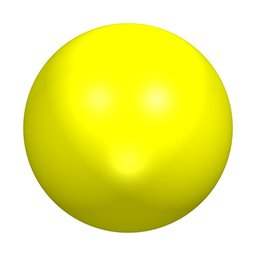
\includegraphics[width=1.1cm]{./../../common/images/kugel}
        \end{tabular}
        &
        \begin{tabular}{@{}c@{}}
          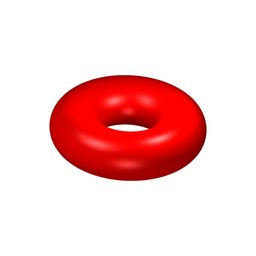
\includegraphics[width=1.1cm]{./../../common/images/torus}
        \end{tabular}
        &
        \begin{tabular}{@{}c@{}}
          带奇点:
        \end{tabular}
        &
        \begin{tabular}{c@{}@{}}
          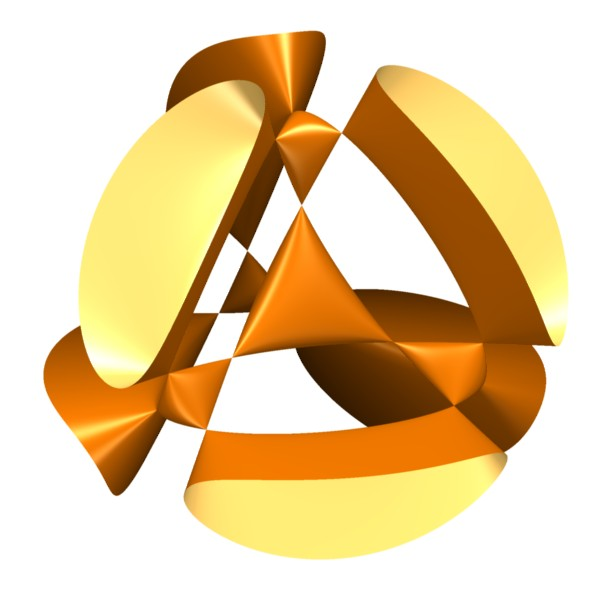
\includegraphics[width=1cm]{./../../common/images/kummer}
        \end{tabular}
        &
        \begin{tabular}{c@{}@{}}
          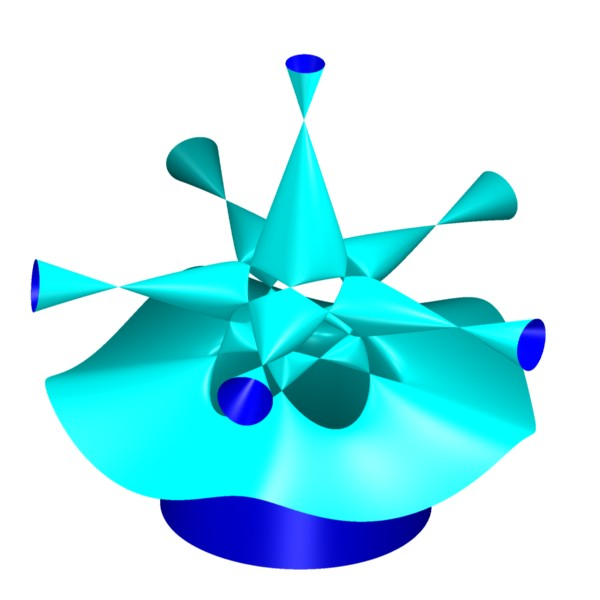
\includegraphics[width=1cm]{./../../common/images/togliatti}
        \end{tabular}
        &
        \begin{tabular}{c@{}@{}}
          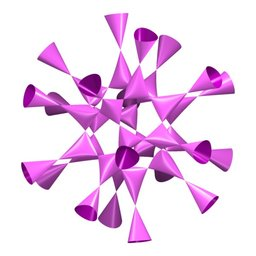
\includegraphics[width=1cm]{./../../common/images/barth_sextic}
        \end{tabular}
      \end{tabular}
    \end{center}
    \vspace{-0.2cm}

所以,带有奇异点的曲面是很特殊的。奇异点是曲面上非常有意思的点。SURFER 项目中的曲面是由多项式定义的。一个多项式的最高项的次数称为多项式的次数。
数学家考虑如下问题:一个固定次数的曲面最多会有多少奇异点?我们把这个数目表示为$\mu(d)$。实践表明,这个数$\mu(d)$非常难以计算。当$d=1,2,3,4$时,19世纪的人们已经知道$\mu(d)$的具体值。但是直到1980年,人们才计算出$\mu(5)$.
$\mu(6)$是1996年被计算出来的。而 $d\ge 7$以及更一般的 $\mu(d)$ 仍然是个未知数。所以关于$\mu(d)$的任何新结果都是非常有重要的。看起来对所有$d$解决这个问题将需要相当长的时间。下面是一些已经知道的结果:
   \begin{center}
      \begin{tabular}{r|cccccccc|c}
        $d$ & $1$ & $2$ & $3$ & $4$ & $5$ & $6$ & $7$ & $8$ & $d$\\
        \hline
        \hline
        \rule{0pt}{1.2em}$\mu(d)\ge$ & $0$ & $1$ & $4$ & $16$ & $31$ & $65$ &
        $99$ & $168$ &
        $\approx \frac{5}{12}d^3$\\[0.3em]
        \hline
        \rule{0pt}{1.2em}$\mu(d)\le$ & $0$ & $1$ & $4$ & $16$ & $31$ & $65$ &
        $104$ & $174$ & $\approx \frac{4}{9}d^3$
      \end{tabular}
    \end{center}
\end{surferIntroPage}
